% ! TeX root = ../../thesis.tex
\chapter{Analisi e Progettazione}
\label{chapter:analysis}
In questo secondo capitolo viene presentata l'analisi dei requisiti e il \textit{design} del sistema.

\section{Requisiti}
Come già anticipato, lo scopo della tesi è realizzare un sistema antiplagio automatico in grado d'individuare eventuali porzioni di codice copiato nei progetti \textit{software} del corso di Programmazione ad Oggetti dell'Università di Bologna.

Di seguito vengono descritti, per punti, i requisiti del sistema, suddivisi tra requisiti \textit{funzionali} e \textit{non funzionali}.

\subsection*{Requisiti funzionali}
\begin{itemize}
    \item Il sistema riceve in \textit{input} un insieme di progetti di cui si vuole verificare l'autenticità, detto \textbf{\textit{Submission}}, e un insieme di progetti con cui confrontarli, detto \textbf{\textit{Corpus}};
    
    \item Il confronto viene effettuato tra progetti sviluppati nello stesso linguaggio di programmazione.
    
    \item I progetti sono sviluppati in linguaggio Java e mantenuti in \textit{repository} pubbliche su \textit{GitHub} e \textit{Bitbucket}\footnote{
        \href{https://github.com}{\textit{GitHub}} e \href{https://bitbucket.org}{\textit{Bitbucket}} sono due tra i più conosciuti servizi di \textit{hosting} per progetti \textit{software} che utilizzano sistemi di controllo di versione decentralizzati, come \href{https://git-scm.com}{Git}.
    }. Si assume che i progetti passati siano tempo-invarianti: dal momento in cui vengono corretti, le rispettive \textit{repository} sono archiviate e mai più modificate;

    \item Il sistema deve fornire in \textit{output} le sezioni di codice che, con un determinato livello di accuratezza, ha stabilito essere simili.
\end{itemize}

\subsection*{Requisiti non funzionali}
\begin{itemize}
    \item L'algoritmo per determinare la similarità, così come le metriche utilizzate, devono essere interscambiabili e facilmente estendibili;
    \item Le informazioni estrapolate dai sorgenti sono salavate in modo tale da essere riutilizzate nelle analisi successive di altri progetti;
    \item \`E necessario che il sistema impieghi un tempo "ragionevole" per effettuare la computazione;
\end{itemize}

\section{Analisi e modello del dominio}
% descrizione session?
Il sistema deve essere in grado, a partire da un insieme di \textit{repository}, corrispondenti a progetti coerenti per linguaggio di programmazione, di estrarne una rappresentazione confrontabile (\textit{SourceRepresentation}) medianti opportuni algoritmi di analisi (\textit{Analyzer}).
%
Ciascuna coppia di rappresentazioni intermedie deve essere successivamente confrontata da algoritmi di rilevamento di somiglianze (\textit{PlagiarismDetector}) al fine di poter determinare eventuali parti di codice duplicato e/o somiglianze, generando infine dei \textit{report}.

Gli elementi costitutivi il problema sono sintetizzati in \Cref{img:02-domain}.

La principale difficoltà sarà individuare tecniche di analisi e di rilevamento delle somiglianze che siano robuste, ovvero permettano d'identificare casi dii copiature anche se lo sviluppatore ha effettuato modifiche per oscurarle.
%
Particolare attenzione dovrà essere posta sulla progettazione dei componenti per l'analisi e per il confronto, in quanto, data la natura del sistema, possono dover cambiare frequentemente ed essere fortemente configurabili.
%
Inoltre, il requisito non funzionale sulle \textit{performance} richiederà un'analisi dei tempi di esecuzione non appena il sistema sarà completato.

\begin{figure}[h!]
    \centering
    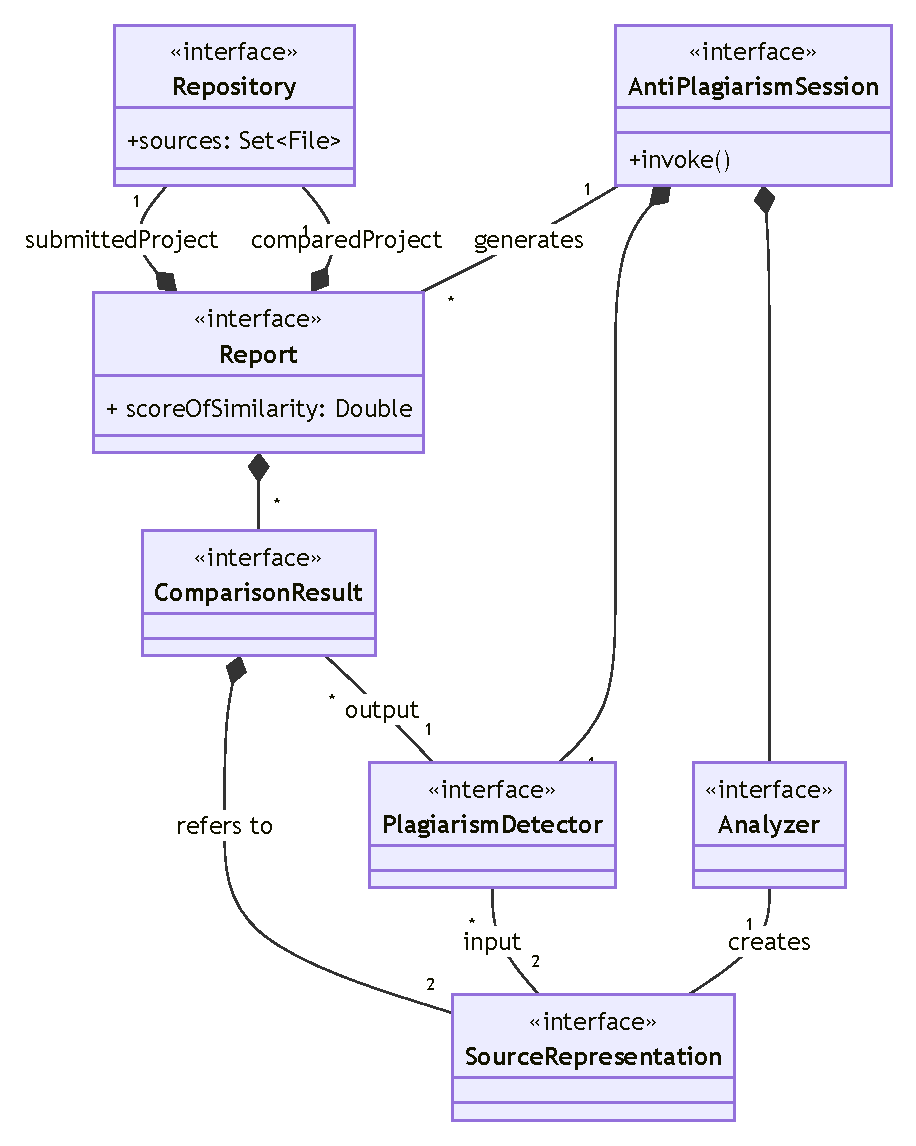
\includegraphics[width=0.8\textwidth]{resources/img/02-domain.pdf}
    \caption{Schema UML delle classi dell'analisi del problema, con rappresentate le entità principali ed i rapporti fra loro.}
    \label{img:02-domain}
\end{figure}

\section{Design}
